\documentclass[language=german,style=solution]{smo}

\usepackage{tikz}
\usetikzlibrary{patterns}
\usetikzlibrary{decorations.pathreplacing}

\place{Zürich}
\examdate{2015}

\title{IMO-Selektion - Musterlösung}

\begin{document}

\begin{enumerate}

\item[\textbf{1.}] %% Exercise 1 %%
Sei $n$ eine natürliche Zahl. Was ist die maximale Anzahl $1\times 1$ Quadrate, die man in einem $n\times n$ Quadrat schwarz färben kann, sodass in jedem $2\times 2$ Quadrat höchstens 2 kleine Quadrate schwarz gefärbt sind?

\textit{Lösung}

\begin{itemize}
\item \underline{$n \equiv 0 \mod{2}$:} Dieser Fall ist relativ simpel: Wir bedecken das Feld mit $2\times 2$ Feldern. In jedem dieser Felder darf es gemäss Voraussetzung maximal $2$ schwarze Felder haben. Wenn wir immer die unteren zwei Felder schwarz färben, bekommen wir eine gültige Färbung:
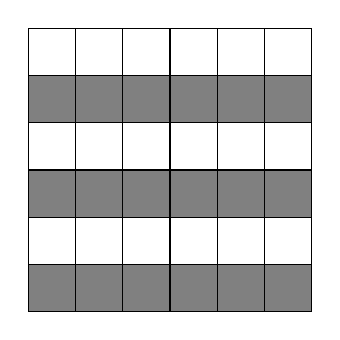
\begin{tikzpicture}[scale=0.6]
\fill[color=black!50] (0,4) rectangle (6,5);
\fill[color=black!50] (0,2) rectangle (6,3);
\fill[color=black!50] (0,0) rectangle (6,1);
\draw (0,0) grid (6,6);
\end{tikzpicture}

\item \underline{$n \equiv 1 \mod{2}$:} Behauptung: Wir können maximal
\[
n\cdot \frac{(n+1)}{2}
\]
Felder schwarz färben.

Konstruktion: Wir färben jede zweite Zeile schwarz

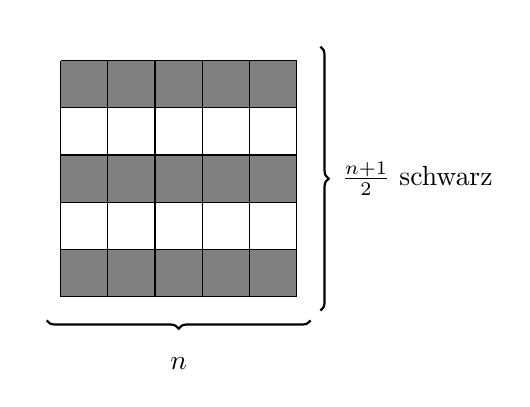
\begin{tikzpicture}[scale=0.6]
\node (n1) at (5.5,-0.5) {};
\node (n3) at (5.5,5.5) {};
\node (s1) at (-0.5,-0.5) {};
\node (s3) at (5.5,-0.5) {};
\fill[color=black!50] (0,4) rectangle (5,5);
\fill[color=black!50] (0,2) rectangle (5,3);
\fill[color=black!50] (0,0) rectangle (5,1);
\draw (0,0) grid (5,5) ;
\draw[thick,decorate,decoration={brace,amplitude=3pt}]
            (n3) -- (n1) node[midway, right=4pt] {$\frac{n+1}{2}$ schwarz};
\draw[thick,decorate,decoration={brace,amplitude=3pt}]
            (s3) -- (s1) node[midway, yshift=-0.55cm] {$n$};
\end{tikzpicture}

Obere Schranke: Wir zeigen die Schranke induktiv. Das heisst, wir nehmen ein $n \times n$ Feld und fügen einen neuen Rand mit Breite 2 hinzu. Wir zeigen, dass wir dann nicht mehr als $(n+2) \frac{(n+2)+1}{2}$ Felder schwarz färben können.\\
Wir bedecken dafür den neuen Rand mit $2 \times 2$ Feldern und einem $1 \times 1$ Feld, wie in folgendem Bild:

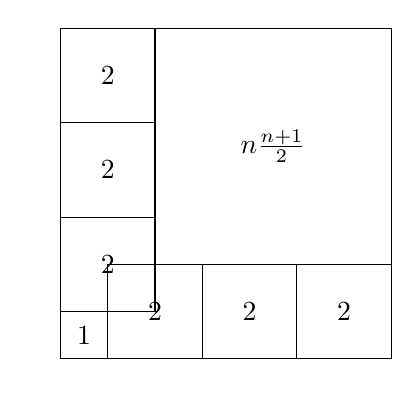
\begin{tikzpicture}[scale=0.6]
\node (n1) at (5.5,-0.5) {};
\node (n3) at (5.5,5.5) {};
\node (s1) at (-0.5,-0.5) {};
\node (s3) at (5.5,-0.5) {};

\draw (0,0) rectangle (7,7);
\draw (2,2) rectangle (7,7);
\draw (0,5) rectangle (2,7);
\draw (0,3) rectangle (2,5);
\draw (0,1) rectangle (2,3);
\draw (1,0) rectangle (3,2);
\draw (3,0) rectangle (5,2);
\draw (5,0) rectangle (7,2);

\draw (2,1) node{2};
\draw (4,1) node{2};
\draw (6,1) node{2};
\draw (1,2) node{2};
\draw (1,4) node{2};
\draw (1,6) node{2};
\draw (0.5,0.5) node{1};
\draw (4.5,4.5) node{$n \frac{n+1}{2}$};
\end{tikzpicture}

\begin{itemize}
\item Es gibt insgesamt $2 \frac{n+1}{2}$ Quadrate der Grösse $2\times 2$ (die Seiten sind $n+2$ lang). In jedem können maximal 2 Felder schwarz sein, also maximal $4 \frac{n+1}{2}$.
\item Im $1 \times 1$ Feld kann maximal 1 Feld schwarz sein.
\item Im grossen Rechteck können maximal $n \frac{n+1}{2}$ schwarz sein (Induktionsannahme).
\end{itemize}

Zusammen ergibt dies eine maximale Anzahl von 
\begin{align*}
4\frac{n+1}{2} + 1 + n \frac{n+1}{2} &= \frac{4n+4}{2} + \frac{2}{2} + \frac{n^2+n}{2}\\
&= \frac{n^2+5n+6}{2}\\
&= \frac{(n+2)(n+3)}{2}\\
&= (n+2) \frac{(n+2)+1}{2}
\end{align*}
Damit ist der Induktionsschritt vollendet.

\end{itemize}

\textit{Marking Scheme}
\begin{itemize}
\item +1 Punkt für $n \equiv 0 \mod(2)$
\item +6 Punkte für $n \equiv 1 \mod(2)$
\end{itemize}

\newpage

\item[\textbf{2.}] %% Exercise 2 %%
Seien $a,b,c \in \R$ mit $a,b,c\geq 1$. Zeige, dass gilt:
\[
\min \left(\frac{10a^2-5a+1}{b^2-5b+10},\, \frac{10b^2-5b+1}{c^2-5c+10},\, \frac{10c^2-5c+1}{a^2-5a+10}\right )\leq abc.
\]

\textit{Solution:}\\
Nous étudions d'abord le cas $a=b=c$. L'inéquation à prouver dans ce cas est 
\[
	\frac{10a^2-5a+1}{a^2-5a+10}\leq a^3 \Leftrightarrow 10a^2-5a+1\leq a^5-5a^4+10a^3 \]
\[	\Leftrightarrow a^5-5a^4+10a^3-10a^2+5a-1 \geq 0 \Leftrightarrow (a-1)^5 \geq 0
\]
qui est vraie car $a\geq 1$.

Nous prouvons maintenant le cas général: 
\begin{align*}
	&\min \left(\frac{10a^2-5a+1}{b^2-5b+10},\frac{10b^2-5b+1}{c^2-5c+10},\frac{10c^2-5c+1}{a^2-5a+10}\right )\\
	&\leq\sqrt[3]{\frac{10a^2-5a+1}{b^2-5b+10}\cdot\frac{10b^2-5b+1}{c^2-5c+10}\cdot\frac{10c^2-5c+1}{a^2-5a+10}}\\
	&= \sqrt[3]{\frac{10a^2-5a+1}{a^2-5a+10}\cdot\frac{10b^2-5b+1}{b^2-5b+10}\cdot\frac{10c^2-5c+1}{c^2-5c+10}}\\
	&\leq\sqrt[3]{a^3\cdot b^3\cdot c^3} = abc
\end{align*}
Où la première inégalité est l'inégalité min-GM et la deuxième inégalité a été prouvée à la première étape.

\textit{Marking Scheme:}
\begin{itemize}
\item +3P für min-GM
\item +3P für $\frac{10a^2-5a+1}{a^2-5a+10}\leq a^3$
\item -1P, falls man $10a^2-5a+1 \geq 0$ nicht gezeigt hat
\item -1P, falls man $a^2-5a+10 > 0$ nicht gezeigt hat
\end{itemize}
\newpage

\item[\textbf{3.}] %% Exercise 3 %%
Sei $ABC$ ein Dreieck mit $AB > AC$ und sei $M$ der Mittelpunkt der Seite $AC$. Weiter sei $D$ ein Punkt auf der Seite $AB$, sodass $DB = DC$ gilt. Die Parallele zu $BC$ durch $D$ und die Gerade $BM$ schneiden sich im Punkt $K$. Zeige, dass $\angle KCD = \angle DAC$ gilt.

\textit{Lösung:}\\
Sei $\beta=\angle CBA$. Da $DBC$ ein gleichschenkliges Dreieck ist, gilt $\angle CBD=\angle DCB=\beta$. Der Aussenwinkel $\angle CDA$ beträgt somit $2\beta$. Da $KD$ parallel zu $BC$ ist, gilt $\angle CDK=\angle DCB=\beta$, woraus folgt, dass $\angle KDA=\angle CDA-\angle CDK=\beta$. $KD$ ist also die Winkelhalbierende des Winkels $\angle CDA$.\\
Seien $E$ und $F$ die Schnittpunkte der Seiten $AB$ und $BC$ mit der Parallelen zur Seite $AC$ durch $K$. Da $KD$ und $FB$ parallel sind, gibt es eine zentrische Streckung mit Streckzentrum $E$, die $K$ auf $F$ und $D$ auf $B$ abbildet. Aufgrund der Konstruktion gilt $EF:EK=AC:AM=2$, d.h. der Streckfaktor der zentrischen Streckung ist 2. Hieraus folgt aber wiederum, dass $ED=DB=DC$ gilt. Da $KD$ die Winkelhalbierende des Winkels $\angle CDA$ ist, ist $E$ genau die Spiegelung von $C$ an der Geraden $KD$. Daraus folgt nun $\angle KCD=\angle DEK=\angle DAC$ und wir sind fertig.

\includegraphics[width=\textwidth]{Muloe3}

\textit{Marking Scheme}
\begin{itemize}
\item Für die Einführung des Punktes $E$ (als Schnittpunkt oder als Punkt auf $AB$ mit $ED=DB$) und eine Angabe der Strategie (z.B. dass es genügt zu zeigen, dass $ED=DB$ gilt) gab es 3 Punkte.
\end{itemize}

\newpage

\item[\textbf{4.}] %% Exercise 4 %%
Finde alle Paare $(a,b)$ teilerfremder ganzer Zahlen, sodass gilt:
\[
a^2+a = b^3+b.
\]

\textit{Solution} :
Comme $a^2+a\geq -\frac{1}{4}$, on a tout de suite $b^3+b\geq 0$, donc $b\geq 0$. L'équation quadratique $a^2-a-b(b^2+1)=0$, si elle possède des solutions réelles, a toujours une racine positive ou nulle et une autre négative ou nulle. Ainsi, sans perte de généralité, prenons $a\geq 0$ et trouvons toutes les solutions $(a,b)$ avec $a,b\geq 0$. Nous avons vu comment trouver ensuite la solution correspondante avec $a\leq 0$.

On a $a(a+1)=b(b^2+1)$. Comme $a$ et $b$ sont premiers entre eux, $a|b^2+1$ et $b|a+1$. En multipliant ces deux relations, il s'en suit que $ab|(a+1)(b^2+1)$, donc $ab|b^2+a+1$.
\begin{itemize}
\item \underline{1er cas} : $a\leq b$. Alors $b^3+b\geq a^3+a\geq a^2+a$ avec égalité pour $a=b=1$. Le cas $b=1$ nous donne donc deux solutions : $(a,b)=(1,1)$ et $(-2,1)$.
\item \underline{2er cas} : $b=0$. Alors on a aussi deus solutions : $(a,b)=(-1,0)$, $(0,0)$ ne sont pas premiers entre eux.
\item \underline{3er cas} : $a>b>1$. Alors, comme $a$ et $b$ sont positifs, $ab\leq b^2+a+1$, donc $b<a\leq \frac{b^2+1}{b-1}=b+1+\frac{2}{b-1}$.
\begin{itemize}
\item Si $b=2$, l'équation $a^2+a=10$ n'a aucune solution.  
\item Si $b=3$, l'équation $a^2+a=30$ possède deux solutions $5$ et $-6$. Comme $a$ et $b$ sont premiers entre eux, on ne retient que $(a,b)=(5,3)$. 
\item Si $b>3$, on a ainsi $a<b<b+2$, donc $a=b+1$. Or, $b|a+1$, donc $b|2$, et $b\leq 2$, contradiction.
\end{itemize}
\end{itemize}
Ainsi, les seules solutions sont $(a,b)=(1,1),(-2,1),(-1,0),(5,3)$.

\textit{Marking Scheme}
\begin{itemize}
\item 2pt pour s'être réduit au cas où  $(a,b)\geq 0$.
\item +1pt pour traiter les petits cas ($b\leq 3$).
\item +3pt pour traiter le cas $b>3$.
\end{itemize}

\newpage

\item[\textbf{5.}] %% Exercise 5 %%
Sei $ABC$ ein Dreieck. Die Punkte $K, L$ und $M$ liegen auf den Seiten $BC, CA$ und $AB$, sodass sich die Geraden $AK, BL$ und $CM$ in einem Punkt schneiden. Zeige, dass man von den Dreiecken $AML, BKM$ und $CLK$ zwei wählen kann, sodass die Summe ihrer Inkreisradien mindestens so gross ist wie der Inkreisradius des Dreiecks $ABC$.

\textit{Lösung}
Nach Ceva gilt $\frac{AM}{MB}\cdot\frac{BK}{KC}\cdot\frac{CL}{LA}=1$. Wir können oBdA annehmen, dass $\frac{BK}{KC}\geq 1$ gilt. Wir unterscheiden nun zwei Fälle. Entweder ist $\frac{CL}{LA}\leq 1$, oder es gilt $\frac{CL}{LA}>1$.

\textbf{1. Fall:} Sei $X$ der Schnittpunkt der Paralllen zu $BC$ durch $M$ und der Seite $AC$, und sei $Y$ der Schnittpunkt der Parallelen zu $AC$ durch $M$ und der Seite $BC$. Wegen $\frac{AX}{XC}=\frac{AM}{MB}=\frac{KC}{BK}\cdot\frac{LA}{CL}\leq \frac{LA}{CL}$ gilt $AX\leq AL$, woraus folgt, dass der Inkreisradius des Dreiecks $AML$ mindestens so gross ist wie der Inkreisradius $r_1$ des Dreiecks $AMX$. Analog erhalten wir aus $\frac{BY}{YC}=\frac{BM}{MA}=\frac{BK}{KC}\cdot\frac{CL}{LA}\leq \frac{BK}{KC}$, dass $BY\leq BK$ gilt und somit der Inkreisradius des Dreiecks $BKM$ mindestens so gross ist wie der Inkreisradius $r_2$ des Dreiecks $BYM$.\\
Es genügt nun zu zeigen, dass $r_1+r_2\geq r$ gilt. Wir werden beweisen, dass $r_1+r_2=r$ gilt. Da $MX$ parallel zu $BC$ ist, gibt es eine zentrische Streckung mit Streckzentrum $A$ und Streckfaktor $\frac{AB}{AM}$, die das Dreieck $AMX$ auf das Dreieck $ABC$ abbildet. Somit gilt $r_1=\frac{AM}{AB}r$ und analog $r_2=\frac{MB}{AB}r$. Aufsummieren liefert nun $r_1+r_2=r$ und wir sind fertig.

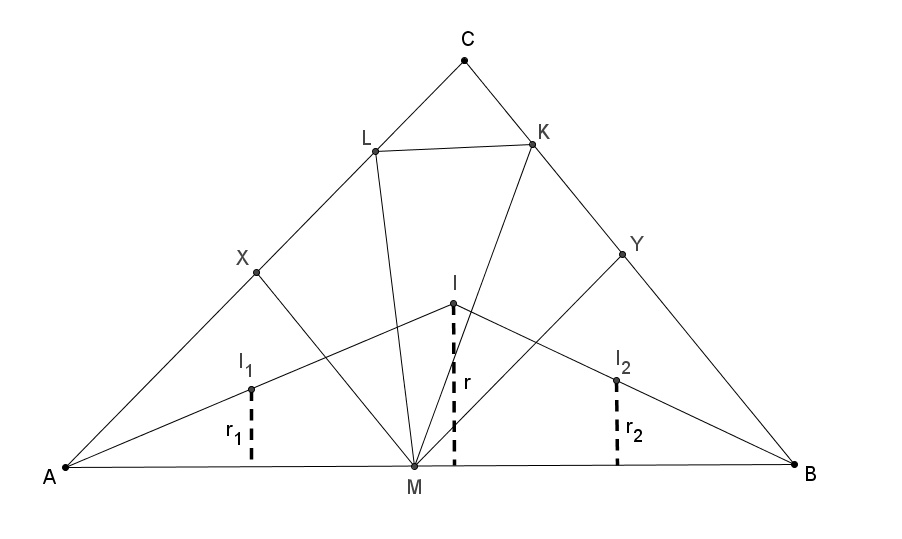
\includegraphics[width=\textwidth]{Muloe5}

\textbf{2. Fall:} Wegen $\frac{BK}{KC},\frac{CL}{LA}\geq 1$ gilt $\frac{AM}{MB}\leq 1$. Dieser Fall ist aber zyklisch symmetrisch zum 1. Fall und funktioniert somit analog.

\textit{Marking Scheme:}
\begin{itemize}
\item 1-2P für Bezug zwischen Ceva und welche Dreiecke wie aussehen.
\item +1P Abschätzung $r_{AML} \geq r_1$
\item +2P Abschätzung der Form $r_1 \geq X \cdot r$
\end{itemize}

\newpage

\item[\textbf{6.}] %% Exercise 6 %%
Finde alle Polynome $P$ mit reellen Koeffizienten, sodass folgende Gleichung für alle $x \in \R$ gilt:
\[
P(x)P(x+1) = P ( x^2 + 2).
\]

\textit{Lösung:}\\
Zuerst bemerken wir, dass die einzigen konstanten Lösungen $P=0$ und $P=1$ sind. Nehme also an $\deg(P)\geq 1$. Wenn $P(x)=0$ für ein $x\in \mathbb{R}$, dann gilt auch $P(x^2+2)=0$ und da $x^2+2 > x$ für alle $x\in \mathbb{R}$ gilt, würde $P$ somit unendlich viele Nullstellen haben, ein Widerspruch.\\
Somit hat $P$ keine reellen Nullstellen, insbesondere muss $\deg(P)$ also gerade sein. Wenn wir mit $c$ den Leitkoeffizienten von $P$ bezeichnen, muss $c^2=c$ gelten (Gleichung betrachten) und da der Leitkoeffizient nicht $0$ sein kann, gilt $c=1$.

Durch Einsetzten des Ansatz $P(X)=X^2+aX+b$ finden wir die einzige quadratische Lösung $P(X)=X^2-X+2$. Offensichtlich ist dann für jede natürliche Zahl $n$ auch $P(X)=(X^2-X+2)^n$ eine Lösung, und wir zeigen nun, dass das die einzigen Lösungen sind.

Seien also $P,Q$ zwei verschiedene Lösungen mit dem selben Grad und $R = P - Q$. Wir haben bereits gesehen, dass jede Lösung normiert sein muss, folglich gilt $deg(R) < deg(P)=deg(Q).$ Nun haben wir für alle $x \in\mathbb{R}$:
\[
(R(x)+Q(x))(R(x+1)+Q(x+1))=P(x)P(x+1)=P(x^2+2)= R(x^2+2) + Q(x^2+2).
\]
Umformen ergibt
\[
R(x)R(x+1)+R(x)Q(x+1)+R(x+1)Q(x)=R(x^2+2).
\]
Da die Gleichung für alle $x\in\R$ gilt, muss sie auch für die Polynome selbst gelten, was nicht möglich ist, wenn man die Grade der Polynome auf beiden Seiten vergleicht. Somit kann es höchstens eine Lösung für einen fixen Grad geben, welche wir bereits gefunden haben.

\textit{Marking Scheme:}
\begin{itemize}
	\item 1P alle Lösungen finden.
	\item 1P Grad von $P$ gerade, führender Koeffizient 1, Versuch, zu zeigen, dass pro Grad maximal eine Lösung existieren kann.
\end{itemize}

\newpage

\item[\textbf{7.}] %% Exercise 7 %%
Trouver tous les ensembles finis et non-vides $A$ de fonctions $f : \R \rightarrow \R$ tels que :

Pour tous $f_1,f_2 \in A$, il existe $g \in A$ telle que pour tout $x,y \in \R$
\[
f_1(f_2(y)-x)+2x=g(x+y).
\]

\textit{Solution:}
Pour commencer, on montre que $A$ est ensemble de fonctions surjectives. En effet, pour $f\in A$ et $f_1=f_2=f$ on a, avec $x=-y$, 
\[
	f(f(y)+y)=g(0)+2y
\]
et donc $f$ est surjective.\\
De plus, avec $x=0$, on obtient que si $f_1,f_2 \in A$ alors $f_1\circ f_2 \in A$.\\
Comme $A$ est non vide, on prend $f\in A$. Par la remarque précédente, on sait que $f^{(k)} \in A$ pour tout $k\in \N$. Comme $A$ est fini, il existe $k_1>k_2$ tels que $f^{(k_1)}=f^{(k_2)}$. Comme $f^{(k_2)}\in A$, $f^{(k_2)}$ est surjective et donc avec $y=f^{(k_2)}$, on obtient
\[
	f^{(k_1-k_2)}(y)=y, \forall y\in \R
\]
Or $f^{(k_1-k_2)}\in A$, donc $A$ contient l'identité. On vérifie facilement que $A=\{id\}$ est un ensemble possible. Montrons maintenant que $A$ ne peut pas contenir autre chose que l'identité.\\
En posant $x=0$ dans notre condition, on obtient que $g=f_1\circ f_2$ et donc on a que pour tout $f_1,f_2 \in A$
\[
	f_1(f_2(y)-x)+2x=f_1(f_2(x+y))
\]
Si $A$ contenait une fonction $h$ autre que l'identité, avec $f_1=id, f_2=h$ et $y=0$, on aurait
\[
	h(x)=x+h(0) \text{  et donc  } h^{(n)}(x)=x+nh(0)
\]
Comme $A$ est fini et que $h^{(n)}\in A$ pour tout $n\in \N$, on a $h(0)=0$ et donc $h\equiv id$.

\textit{Marking Scheme:}
\begin{itemize}
	\item 0P $f_1\circ f_2 \in A$.
	\item 0P Montrer que $g = f_1\circ f_2$.
	\item 1P $A$ est un ensemble de fonctions surjectives.
	\item 2P Conclure que $id \in A$.
\end{itemize}
\vspace{5mm}	
\begin{itemize}	
	\item 2P Pour $h\in A$ montrer que $h+nh(0)\in A$ et $h(0)=0$.
	\item 1P $h=id$.
\end{itemize}
\vspace{5mm}
\begin{itemize}	
	\item -1P Oublier de vérifier que $A=\{id\}$ est une solution.
\end{itemize}



\newpage

\item[\textbf{8.}] %% Exercise 8 %%
Trouver tous les triplets d'entiers naturels $(a,b,c)$ tels que pour tout entier naturel $n$ qui n'a pas de diviseur premier plus petit que $2015$
\[
n+c \div a^n+b^n+n.
\]

\textit{Solution:}\\
\textbf{Lemme} - Il existe une infinité de nombres premiers $p$ tel que $p\equiv 2 \pmod 3$.\\
\textit{Démonstration} : Par l'absurde, soient $p_1,...,p_n$ les uniques premiers congrus à $2$ modulo $3$. \\
Si $n$ est pair, alors $p_1p_2...p_n+1\equiv 2 \pmod 3$ et donc ce nombre possède au moins un diviseur premier $q\equiv 2\pmod 3$. Or, il n'est divisible par aucun des $p_i$.\\
Si $n$ est impair, alors $p_1p_2...p_n+3\equiv 2 \pmod 3$ et on conclut de même.

On prend un nombre premier $p>\max(|a+b-c|,a,b,2015)$ et un entier $n$ tel que :
\begin{align*}
n &\equiv -c \pmod p \\
n &\equiv 1 \pmod {p-1} \\
n &\equiv 1 \pmod {p_i} \text{ pour } p_i<2015 \text{ tel que } (p-1,p_i)=1
\end{align*}
Ce système possède une solution par le thérorème des restes chinois. De plus, le $n$ solution n'est divisible par aucun nombre premier inférieur à $2015$, car si $q<2015$, alors soit $q|p-1$ mais $(n,p-1)=1$, soit $(q,p-1)=1$ mais alors $n \equiv 1 \pmod {q}$. De plus, par construction, $p|n+c$. On peut donc substituer ce $n$ dans l'équation. On a alors 
\[
a^n+b^n+n \equiv a+b+n \equiv a+b-c \equiv 0 \pmod p
\]
La première égalité vient du petit théorème de Fermat. En effet, comme $p>a,b$, on a $(a,p)=(b,p)=1$ et comme $n \equiv 1 \pmod {p-1}$, on a $a^n=a^{k(p-1)+1} \equiv a \pmod p$.\\
Donc $|a+b-c|$ est divisible par $p$, mais $p>|a+b-c|$, donc $a+b=c$.

On réitère le processus avec un premier $p>\max(|a^3+b^3-a-b|,a,b,2015)$, $p\equiv 2 \pmod 3$ et un entier $n$ tel que :
\begin{align*}
n &\equiv -a-b \pmod p \\
n &\equiv 3 \pmod {p-1} \\
n &\equiv 1 \pmod {p_i} \text{ pour } p_i<2015 \text{ tel que } (p-1,p_i)=1
\end{align*}
On a alors
\[
  a^n+b^n+n \equiv a^3+b^3+n \equiv a^3+b^3-a-b \equiv 0 \pmod p
\]
Et donc, $a+b=a^3+b^3$ avec égalité si et seulement si $a=b=1$. On a donc l'unique solution $(1,1,2)$, dont on vérifie trivialement que c'est une solution.

\textit{Marking Scheme:}
\begin{itemize}
	\item 1-2P Familie nützlicher Zahlen finden, indem man $p$ gross wählt.
	\item 2P von Teilbarkeit zu Gleichung kommen.
	\item 2P verschiedene Gleichungen haben.
\end{itemize}

\newpage

\item[\textbf{9.}] %% Exercise 9 %%
Sei $n \geq 2$ eine natürliche Zahl. In der Mitte eines kreisförmigen Gartens steht ein Wachturm. Am Rand des Gartens stehen $n$ gleichmässig verteilte Gartenzwerge. Auf dem Wachturm wohnen aufmerksame Wächter. Jeder Wächter überwacht einen Bereich des Gartens, der von zwei verschiedenen Gartenzwergen begrenzt wird.\\
Wir sagen, dass Wächter $A$ den Wächter $B$ kontrolliert, falls das gesamte Gebiet von $B$ in dem von $A$ enthalten ist.\\
Unter den Wächtern gibt es zwei Gruppen: Lehrlinge und Meister. Jeder Lehrling wird von genau einem Meister kontrolliert und kontrolliert selbst niemanden, während Meister von niemandem kontrolliert werden.\\
Der ganze Garten hat Unterhaltskosten:
\begin{itemize}
\item Ein Lehrling kostet 1 Goldstück pro Jahr.
\item Ein Meister kostet 2 Goldstücke pro Jahr.
\item Ein Gartenzwerg kostet 2 Goldstücke pro Jahr.
\end{itemize}
Zeige, dass die Gartenzwerge mindestens so viel kosten wie die Wächter.

\textit{Lösungen:}
Wir nennen den Bereich zwischen zwei Gartenzwergen ein Interval. Definiere eine Kette als ein $n-1$-Tupel von Intervallen $(I_1,\dots,I_{n-1})$, wobei $I_1 \subset I_2\subset\dots \subset I_{n-1}$ und alle Inklusionen strikt sind.

\textbf{Lemma:} Jedes Intervall ist in genau $2^{n-2}$ Ketten enthalten.

Sei $I$ das gegebene Intervall. Nummeriere die Gartenzwerge im Uhrzeigersinn von $1$ bis $n$ und bezeichne mit $(a,b)$ das Intervall, welches im Uhrzeigersinn von Gartenzwerg $a$ bis zu Gartenzwerg $b$ geht, wobei $1\leq a,b\leq n$ und $a\neq b$. Wir können o.B.d.A. annehmen, dass $I=(1,a)$ mit $1<a\leq n$. Für jede Kette $(I_1,\dots,I_{n-1})$ welche $I$ enthält, muss $I = I_{a-1}$ gelten. Somit haben wir zwei Möglichkeiten für $I_a$ (falls $a \neq n$), nämlich $(1,a+1)$ oder $(n,a)$. Mit der selben Überlegung für $I_a$ etc. findet man schliesslich, dass es $2^{n-a}$ Möglichkeiten gibt, die Kette nach Oben zu vervollständigen. Analog gibt es $2^{a-2}$ Möglichkeiten, die Kette nach unten zu vervollständigen und somit insgesamt $2^{n-2}$ Ketten, welche $I$ enthalten.
Sei nun $M$ und $L$ die Anzahl Meister bzw. Lehrlinge. 

Da pro Kette höchstens ein Intervall eines Meisters enthalten ist, ist die Anzahl Ketten, welche ein Intervall eines Meisters enthalten $M2^{n-2}$.
Als nächstes zählen wir die Anzahl Ketten, welche das Intervall eine Lehrlings aber keines eines Meisters enthalten. Nach Aufgabenstellung gibt es für einen fixen Lehrling genau ein Intervall, welches nicht in der Kette vorkommen darf. Mit den selben Überlegungen wie im Lemma gibt es somit $L2^{n-3}$ solche Ketten. Schliesslich ist die gesamt Anzahl ketten, wieder wegen dem Lemma,  $n2^{n-2}$ und wir erhalten die Ungleichung  $n2^{n-2} \geq M2^{n-2}+L2^{n-3}$. Dies ist äquivalent zu $2n \geq 2M +L$, was wir zeigen wollten.

\textit{Marking Scheme:} Dimitri fragen.

\newpage

\item[\textbf{10.}] %% Exercise 10 %%
Sei $ABCD$ ein Parallelogramm. Nehme an, es existiere ein Punkt $P$ im Innern des Parallelogramms, der auf der Mittelsenkrechten von $AB$ liegt und sodass $\angle PBA=\angle ADP$ gilt.\\
Zeige, dass $\angle CPD=2 \,\angle BAP$ gilt.

\textit{1. Lösung:}
Wir verschieben das Dreieck $ABP$ um den Vektor $\vec{AD}$, das heisst $A$ kommt auf $D$ und $B$ auf $C$ zu liegen. Der Punkt $P$ wird auf den Punkt $P'$ abgebildet, sodass $PP'=AD$ gilt und $PP'$ parallel zu $AD$ ist. Nun gilt:
\[
\angle P'CD=\angle PBA=\angle ADP=\angle P'PD.
\]
Hieraus folgt, dass $PCP'D$ ein Sehnenviereck ist. Mit dem Peripheriewinkelsatz folgt nun:
\[
\angle CPP'=\angle CDP'=\angle BAP.
\]
Damit erhalten wir das gewünschte Resultat:
\[
\angle CPD=\angle CPP'+\angle P'PD=\angle BAP+\angle PBA=2\angle BAP.
\]

\begin{center}
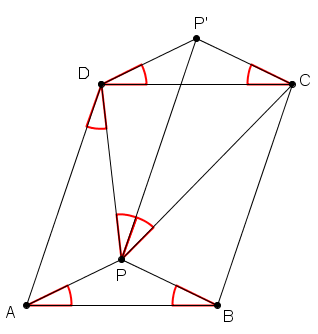
\includegraphics[width=.5\textwidth]{Muloe10_1}
\end{center}

\textit{2. Lösung:}
Sei $M$ der Mittelpunkt des Umkreises $k$ des Dreiecks $APD$. Wegen $\angle BAP=\angle ADP$ ist $AB$ eine Tangente an $k$ und somit stehen $MA$ und $AB$ senkrecht aufeinander. Wir betrachten nun die Spiegelung des Dreiecks $BCP$ an der Mittelsenkrechten von $AB$. Dabei wird $B$ auf $A$ und $P$ auf $P$ abgebildet. Wir möchten zeigen, dass der Bildpunkt $C'$ von $C$ auf $k$ zu liegen kommt. Aufgrund der Konstruktion gilt $C'A=DA$. Ausserdem gilt:
\begin{align*}
	\angle MAC'&=\angle BAC'-\angle BAM\\
	&=\angle CBA-90^\circ\\
	&=180^\circ-\angle BAD-90^\circ\\
	&=\angle BAM-\angle BAD\\
	&=\angle DAM.
\end{align*}
Wir können $C'$ also auch als die Spiegelung von $D$ an der Geraden $AM$ verstehen. Hieraus folgt nun, dass $C'$ ebenfalls auf $k$ liegt. Somit ist $APDC'$ ein Sehenviereck und es gilt $\angle AC'P=\angle ADP$. Winkeljagd liefert uns nun:
\[
\angle CPD=\angle ADP+\angle PCB=\angle ADP+\angle AC'P=2\angle ADP=2\angle BAP.
\]

\begin{center}
    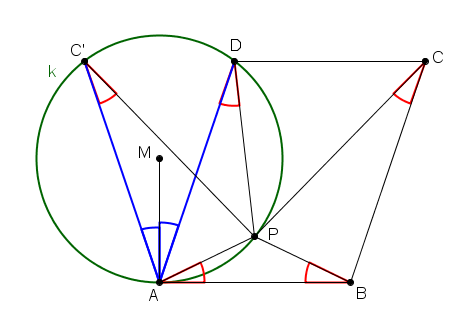
\includegraphics[width=.7\textwidth]{Muloe10_2}
\end{center}

\textit{Marking Scheme}
\begin{itemize}
	\item 2P Behaupten, dass etwas sinnvolles ein Sehnenviereck ist.
	\item +2P dies zeigen
\end{itemize}


\newpage

\item[\textbf{11.}] %% Exercise 11 %%
Im Teil-Land gibt es $n$ Städte. Je zwei Städte sind durch eine Einbahnstrasse verbunden, die entweder nur mit dem Töff oder nur mit dem Auto befahrbar ist. Zeige, dass es eine Stadt gibt, von der aus jede andere Stadt entweder mit dem Töff oder mit dem Auto erreicht werden kann.

\textit{Bemerkung: Es muss nicht jede andere Stadt mit dem gleichen Verkehrsmittel erreicht werden.}

\textit{Lösung:} Wir benützen starke Induktion nach $n$. $n=1$ ist trivial. Betrachte nun $n+1$ Städte $A_0,A_1,\dots,A_n$, welche nach Induktionsvoraussetzung wie folgt geordnet werden können: $A_i$ besitzt die gewünschte Eigenschaft für den Subgraphen induziert durch $A_i,A_{i+1},\dots,A_n$ für $i \ge 1$. Nehme nun an, es gibt keine Stadt mit jener Eigenschaft. Wir konstruieren nun eine unendliche Folge von Städten $A_{k_{i}}$. Falls eine Kante $A_1A_0$ existiert, gibt es einen Widerspruch. OBdA sei $A_0A_1$ mit dem Töff befahrbar. Sei nun $A_{k_0}$ die erste Stadt, welche nicht von $A_0$ durch einen monochromen Weg erreicht werden kann. Nun existiert ein monochromer Weg $A_1\dots A_{k_0}$, welcher mit dem Auto befahrbar sein muss. Entsprechend muss die Kante $A_{k_0}A_0$ mit dem Töff befahrbar sein. Wir definieren unsere Folge induktiv wie folgt: Für $i \ge 1$ sei $A_{k_{i}}$ die erste Stadt, welche von $A_{k_{i-1}}$ nicht mit einem monochromen Weg erreicht werden kann. Wir zeigen induktiv, dass der monochrome Weg $A_{k_{i}}\dots A_{k_0}$ mit dem Töff befahrbar sein muss. Der monochrome Weg $A_0A_{k_i}$ muss mit dem Auto befahrbar sein, sonst existiert ein mit Töff befahrbarer monochromer Weg $A_{k_{i-1}} \dots A_{k_0}A_0\dots A_{k_{i}}$. Es folgt, dass der monochrome Weg $A_{k_i}\dots A_{k_0}$ mit dem Töff befahrbar sein muss. Dies zeigt ferner, dass $k_i \ge 2$  für alle $i$.
Eine solche unendliche Folge kann nicht existieren. Widerspruch.

\textit{Marking Scheme:}
\begin{itemize}
	\item 1P Mit Induktion auf sinnvolles OBdA kommen.
	\item +1-2P sinnvolle Folge definieren/basteln
\end{itemize}


\newpage

\item[\textbf{12.}] %% Exercise 12 %%
Gegeben sind zwei natürliche Zahlen $m$ und $n$. Zeige, dass es eine natürliche Zahl $c$ gibt, sodass jede von $0$ verschiedene Ziffer gleich oft in $cm$ und $cn$ vorkommt.

\textit{Lösung:}
Wir zeigen zuerst, dass es genügt den Fall zu betrachten, wo $n$ teilerfremd zu $10$ ist. Nehme also an die Aufgabe ist für solche $n$ bewiesen und betrachte den Fall wo $n=2^a5^bn'$ mit $(n',10)=1$ und $m$ beliebig. Wegen unserer Annahme gibt es nun ein $c$, so dass in $c(2^b5^am)$ und $cn'$ jede von $0$ verschiedene Ziffer gleich oft vorkommt. Dann gilt dasselbe aber auch für $(c2^b5^a)m$ und $(c2^b5^a)n=10^{a+b}n'$. 
Somit können wir uns auf den Fall beschränken wo $(n,10)=1$ gilt.
Die Idee ist nun eine dritte natürliche Zahl $k$ zu wählen, so dass $cm$ und $cn$ bis auf $0$ genau die Ziffern von $m,n,k$ bzw. $n,k,m$ in dieser Reihenfolge enthalten. In Gleichungen übersetz heisst das
\[
c= 10^t + \frac{10^sn+k}{m} = 10^t + \frac{10^rk+m}{n}.
\]
Damit sich die Ziffernblöcke nicht überschneiden sollten zusätzlich folgende Ungleichungen gelten:
\[
10^r >m, 10^s>k, 10^t>\max\{10^sn+k,10^rk+m\}.
\]
Umformen ergibt 
\[
k=\frac{10^sn^2-m^2}{10^rm-n}.
\]
Damit dies eine ganze Zahl ist, wählen wir zuerst $r$, so dass $10^r>m$ und $10^rm-n>n^2$ gilt. Da $(n,10)=1$ gilt, exisitert nach dem Satz von Euler-Fermat ein $s$ mit
\[
10^{s+2r} \equiv 1 \mod(10^rm-n).
\]
Dann gilt
\[
10^sn^2-m^2\equiv 10^{s+2r}m^2-m^2 \equiv 0 \mod(10^rm-n)
\]
und somit können wir $k$ durch obige Gleichung als natürlich Zahl definieren. Zudem haben wir die Ungleichung
\[
10^s > k \frac{10^rm-n}{n^2} > k.
\]
Schliesslich können wir noch $t$ genügend gross wählen, so dass 
\[
10^t>\max\{10^sn+k,10^rk+m\}
\]
gilt. Nun müssen wir nur noch überprüfen, dass $c$ wie oben definiert ein natürliche Zahl ist, was aus
\[
10^{s+2r} \equiv 1\mod(10^rm-n)
\]
und 
\[
\frac{10^rk+m}{n} = \frac{10^{r+s}n-m}{10^rm-n}\in \N
\]
folgt.

\end{enumerate}

\end{document}
